\section{Référence de la classe CBdd}
\label{class_c_bdd}\index{CBdd@{CBdd}}
Graphe d'héritage de CBdd::\begin{figure}[H]
\begin{center}
\leavevmode
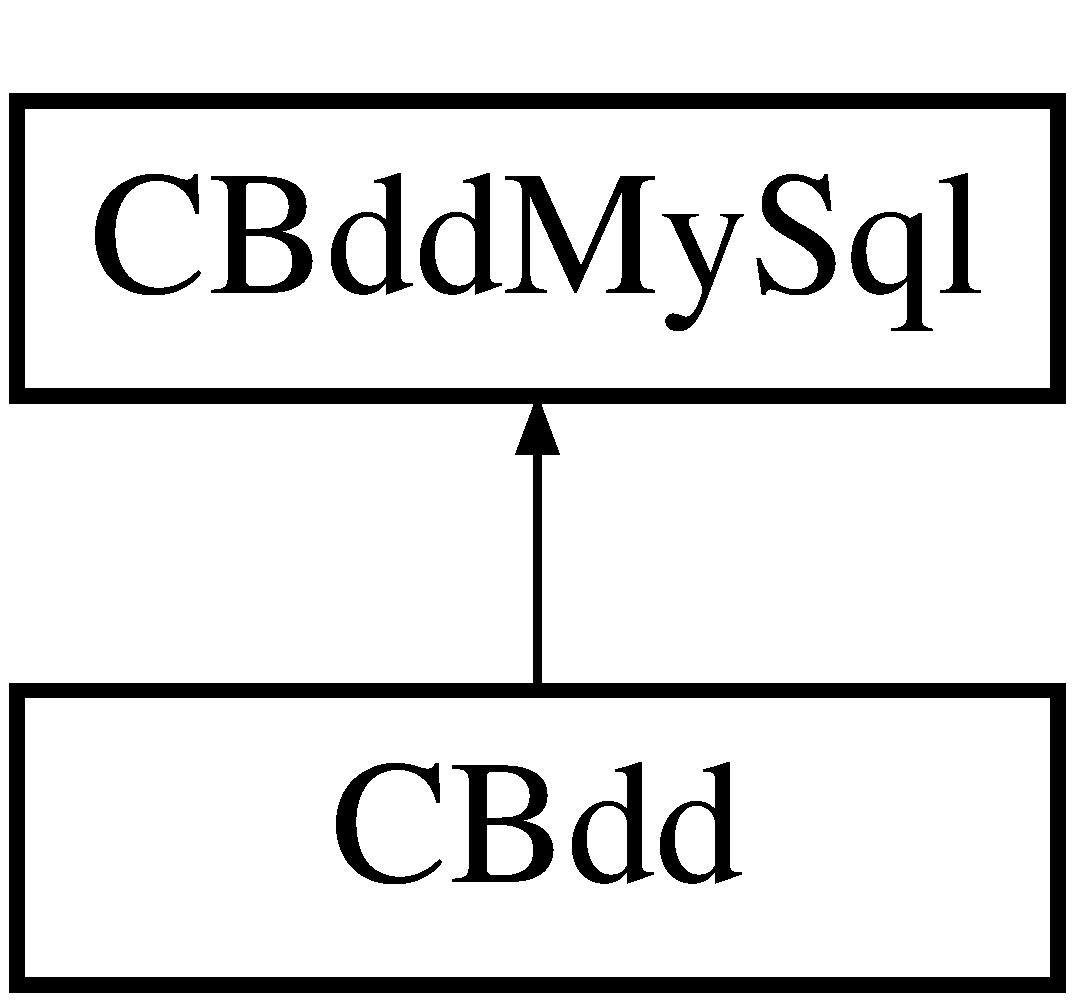
\includegraphics[height=2cm]{class_c_bdd}
\end{center}
\end{figure}


\subsection{Description détaillée}
Gestion de la DB, adaptée à Esprit, utilisant des variables globales du projet (config) pour déterminer les paramètres de connexion. \subsection*{Fonctions membres publiques}
\begin{CompactItemize}
\item 
{\bf CBdd} ()
\begin{CompactList}\small\item\em Constructeur. \item\end{CompactList}\end{CompactItemize}


\subsection{Documentation des fonctions membres}
\index{CBdd@{CBdd}!CBdd@{CBdd}}
\index{CBdd@{CBdd}!CBdd@{CBdd}}
\subsubsection{\setlength{\rightskip}{0pt plus 5cm}CBdd::CBdd ()}\label{class_c_bdd_4f77ce242d778ba4ff89f8c54002b2e6}


Constructeur. 

Effectue une connexion automatique à la DB grâce en utilisant les variables globales de la config comme paramètres 

Références CBddMySql::CBddMySql().

La documentation de cette classe a été générée à partir du fichier suivant :\begin{CompactItemize}
\item 
src/database/{\bf bdd.class.php}\end{CompactItemize}
